\documentclass[assd_tp2_main.tex]{subfiles}

\begin{document}

\section{Síntesis de sonidos mediante modelos f\'isicos}
Se analizarán dos variantes del modelo Karplus-Strong en paralelo, tanto de manera teórica como práctica. 

\subsection{Bloque A Elemental}
Se resolverá, como cálculo auxiliar un bloque sencillo definido como:
\begin{figure}[H]	
	\centering
	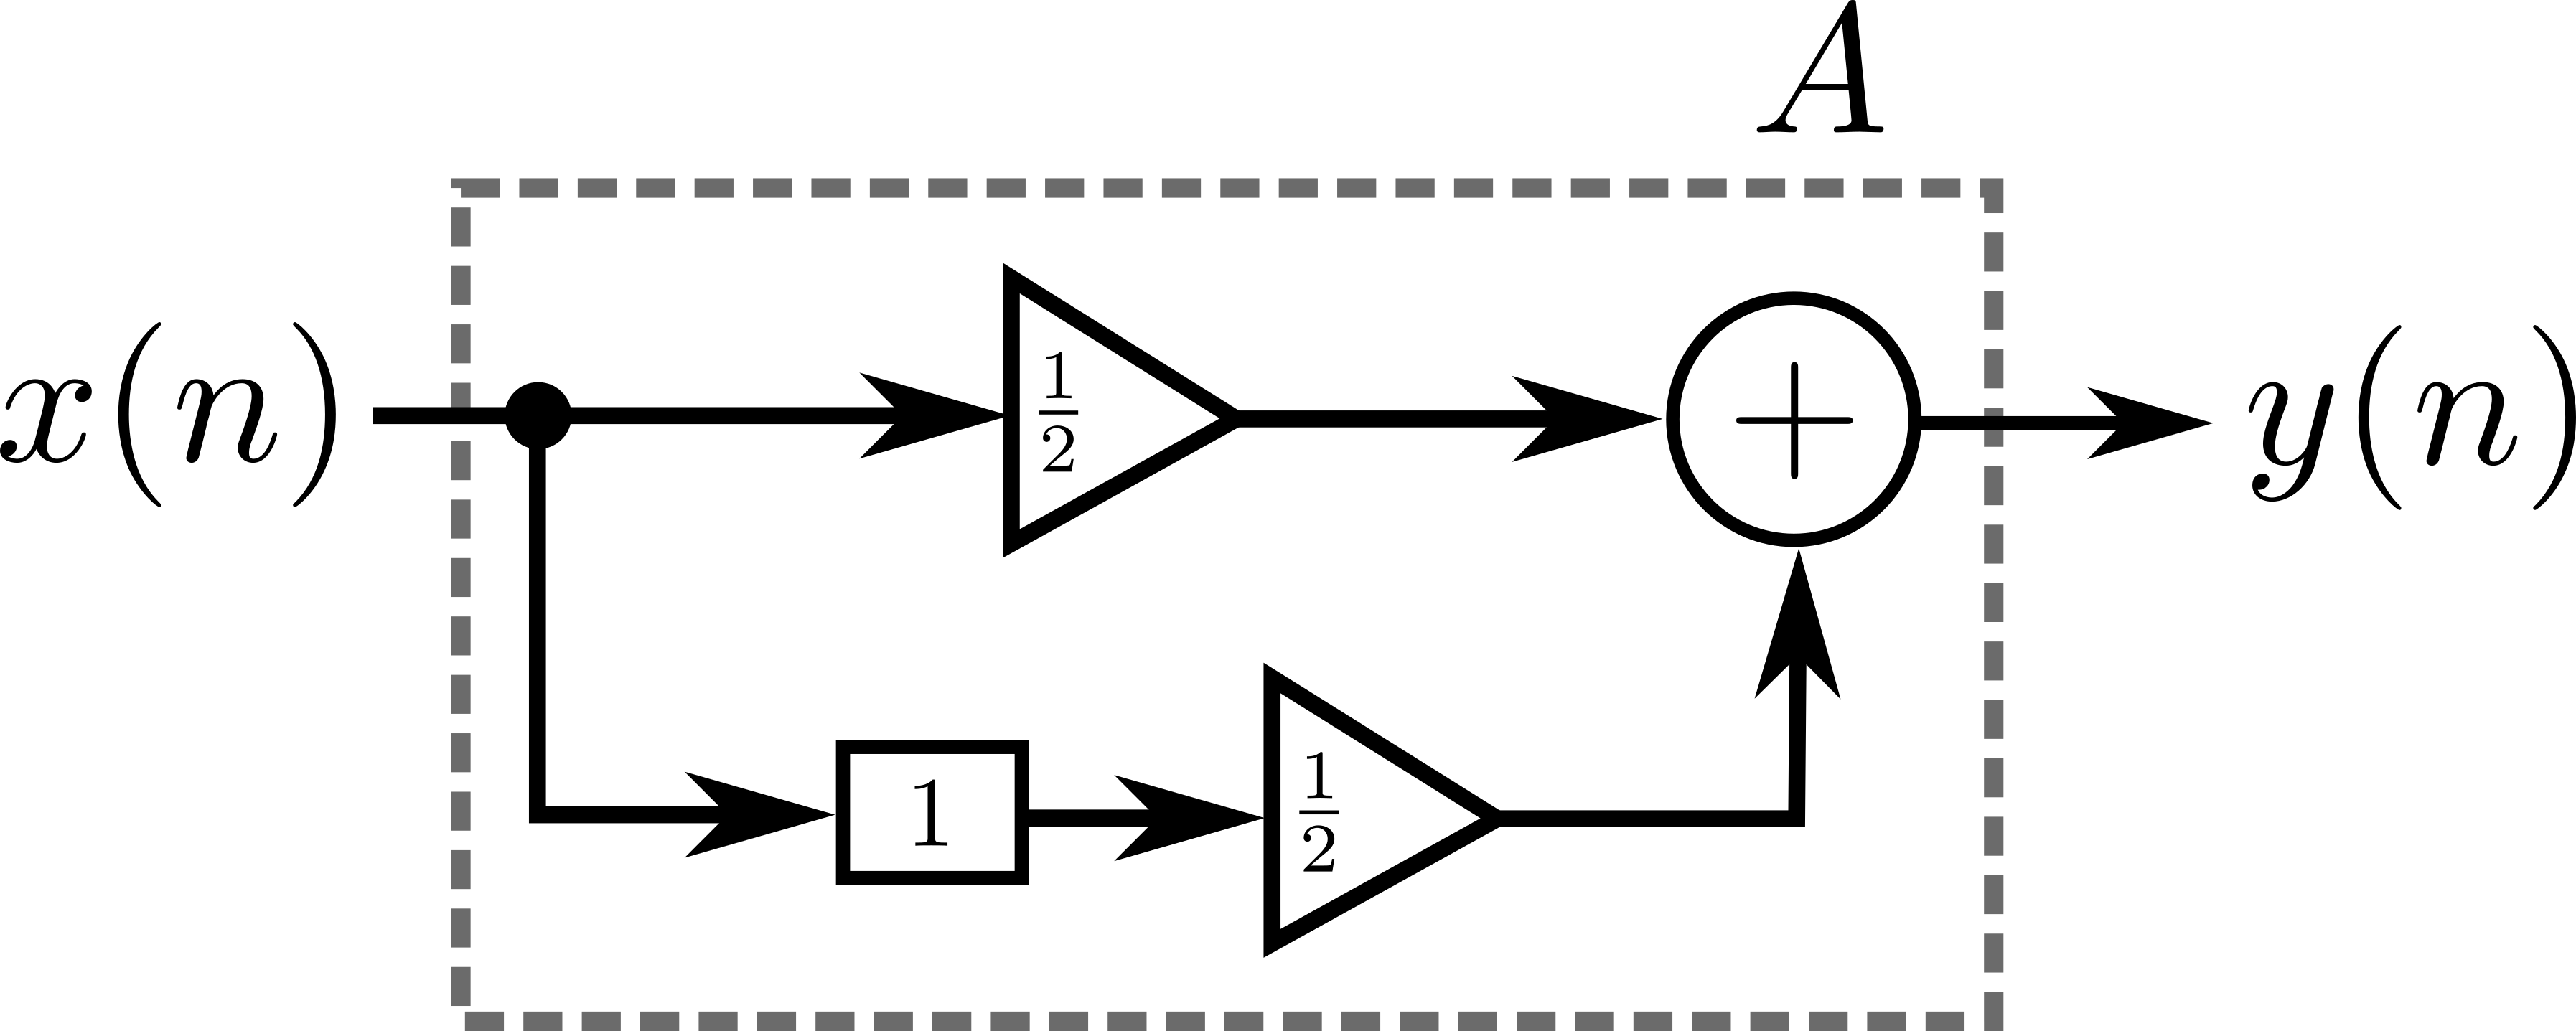
\includegraphics[scale=1]{graficos/bloque1ej5.png}
	\caption{Bloque elemental}
	\label{fig:bloqueElemental}
\end{figure}

Este bloque solo promedia los dos ultimos valores de entrada. Su transferencia esta dada por
\begin{equation}
x(n)=\frac{1}{2}x(n)+\frac{1}{2}x(n-1)
\end{equation}
\begin{equation}
Y(z)=\frac{1}{2}X(z)+\frac{1}{2}X(z)z^{-1} \implies A(z)=\frac{z+1}{z}
\end{equation}
Se puede observar que el bloque A es pasa-bajos (cero en $Z=-1$); lo cual es, en principio, razonable, el bloque A suaviza la entrada.

\subsection{Karplus Strong 1}
\subsubsection{Análisis teórico}
Se resolverá un nuevo sistema, denominado $S_1$, el cuál consiste en una adicion de realimentación al sistema anterior.
\begin{figure}[H]	
	\centering
	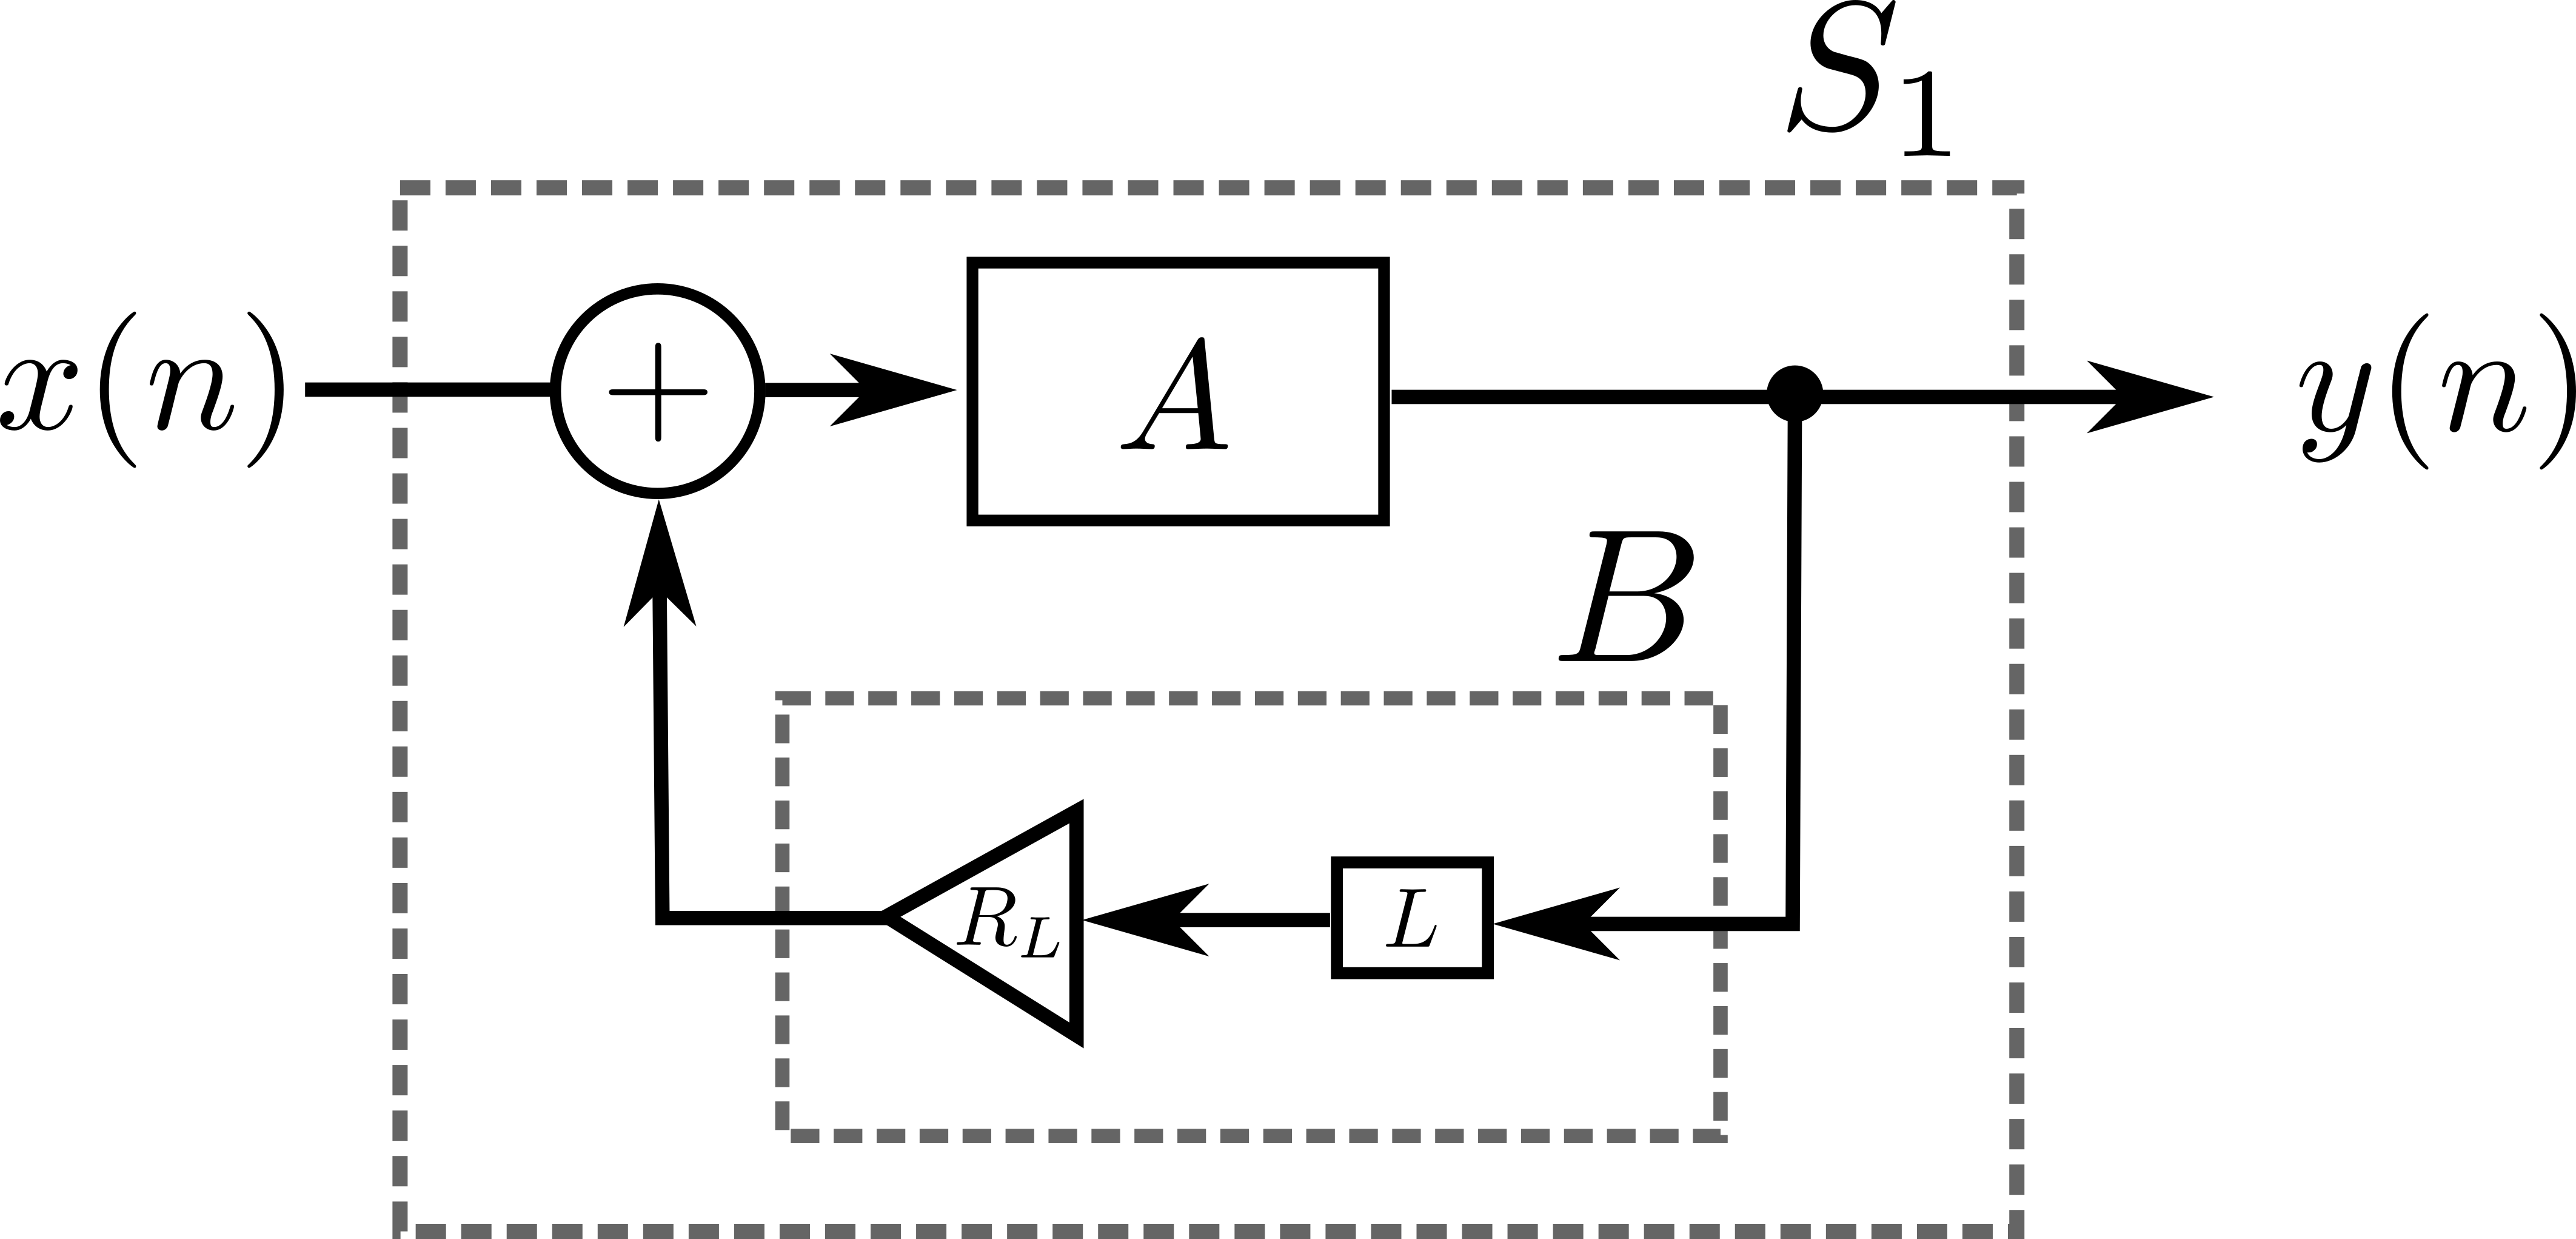
\includegraphics[scale=1]{graficos/bloque2ej5.png}
	\caption{Bloque elemental}
	\label{fig:bloqueElemental}
\end{figure}

Mediante teoria de feedback a considerando que $B(z)=z^{-L}R_L$ se llega a que
\begin{equation}
S_1(z)=\frac{\frac{1}{2}+\frac{1}{2}z^{-1}}{1-\frac{1}{2}R_Lz^{-L}-\frac{1}{2}R_Lz^{-L-1}}=\frac{ \frac{1}{2} z^{L+1} + \frac{1}{2}z^L}{ z^{L+1} - \frac{1}{2}R_L z-\frac{1}{2}R_L } 
\end{equation}
\begin{equation}
y(n)=\frac{1}{2}x(n)+\frac{1}{2}x(n-1)+\frac{1}{2}R_Ly(n-L)+\frac{1}{2}R_Ly(n-L-1)
\end{equation}

Es decir, una expresión con $L+1$ polos y $L+1$ ceros, en otras palabras, una ecuación diferencial de orden $L+1$ con vector de longitud $L$ como condición inicial. De la ecuación de diferencias se puede observar que la unica forma de garantizar estrictamente la estabilidad del sistema será exigiendo $R_L<1$. No obstante, en la práctica como la frecuencia de resonancia del sistema no será exacta; colocar $R_L=1$ no provocará inestabilidad. Más aun; resulta provechoso aproximar $R_L$ a $1$ lo más posible para lograr estirar la duración de las oscilaciones.   

\subsubsection{Estudio de la distribución polos y ceros, respuesta en frecuencia}
\begin{figure}[H]	
	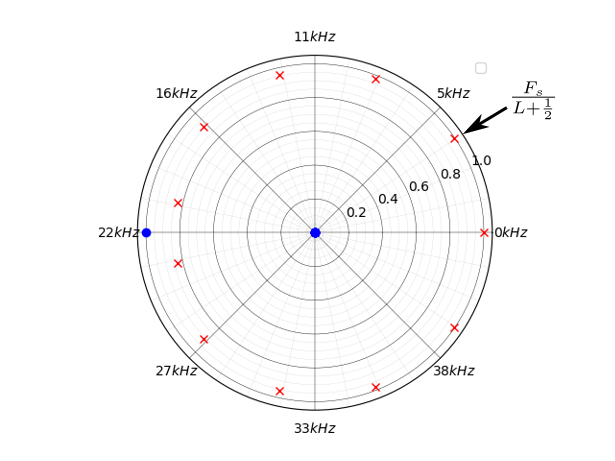
\includegraphics[scale=0.45]{graficos/polos.png}
	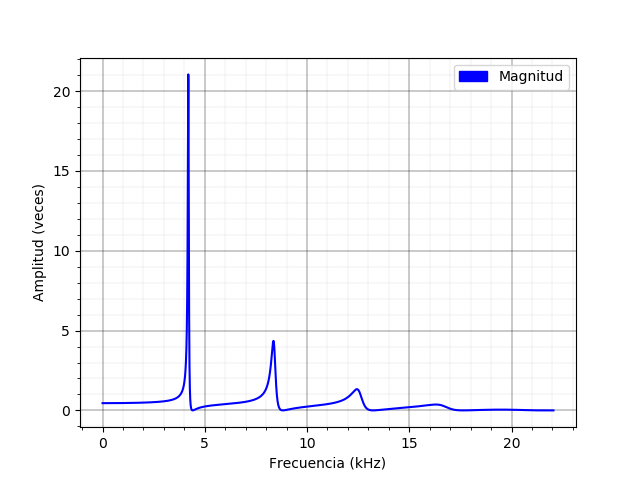
\includegraphics[scale=0.58]{graficos/freq_response.png}
	\caption{Polos y ceros (derecha), Rta en frecuencia (izquierda), $S_1$ con $R_L=1$, $L=10$, $f_s=44.1kHz$}
	\label{fig:polosCeros}
\end{figure}

Del diagrama de polos y ceros y la respuesta en frecuencia podemos observar que hay una frecuencia de resonancia $F_R=F_s/(L+\frac{1}{2})$ que tiende a cumplir las hipotesis del criterio de Barkhausen, y por lo tanto provocar oscilaciones, lo cuál es el objetivo del bloque; conseguir una salida que perdure en el tiempo a partir de una entrada de longitud $L$ muy corta.

\subsubsection{Cálculo de $F_R$}
Se mostrará porque el sistema resuena en $F_R=F_s/(L+\frac{1}{2})$. En la sección anterior se observó que la frecuencia de resonancia debía ser aquella que tendiera a cumlir las hipotesis del criterio de barkhausen; en otras palabras; que la ganancia del lazo se aproxime a $1$ con $0$ grados. 
El sistema esta compuesto por la superposición de un sistema con un retraso de lazo $L$ y otro sistema con retrazo de lazo $L+1$. Por lo tanto; para que una señal no tienda a interferirse al recorrer el lazo debe tener periodo $\frac{L+L+1}{2}$; es decir una frecuencia $\frac{F_s}{L+1/2}$

\subsubsection{Análisis mediante señales}
 
Se procederá a estudiar como el sistema responde a diversas entradas, entre ellas, un impulso unitario, ruido gaussiano de longitud $L$, y ruido lineal de longitud $L$. Se decidió aumentar $L$ en estos casos a $50$ para conseguir frecuencias más cercanas a las audibles.
 
\begin{figure}[H]
	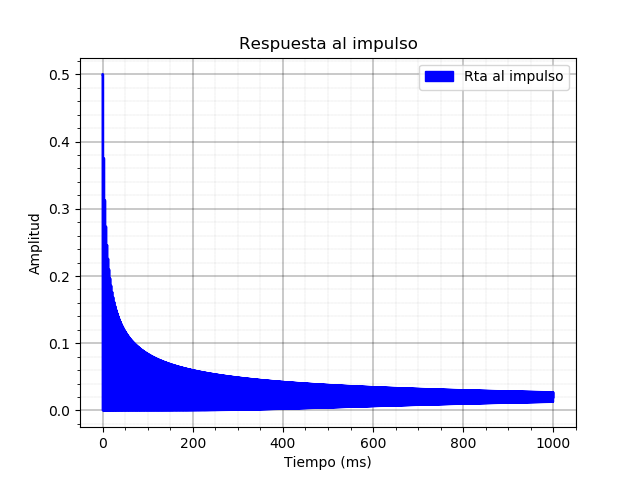
\includegraphics[scale=0.55]{graficos/impulsoBloqueS1.png}
	\includegraphics[scale=0.41]{graficos/impulsoBloqueS1Zoom.png}
	\caption{Respuesta al impulso con y sin zoom, $R_L=1$, $L=50$, $f_s=44.1kHz$}
\end{figure}

Se puede observar que, de todas las frecuencias pertenecientes al impulso, la más amplificada vale $865Hz \approx \frac{F_s}{1/2+L}$. Por otro lado es importante observar que la salida se encuentra montada sobre una tensión continua, más precisamente, nunca es menor que 0. Esto se debe a que cuando la excitación es exclusivamente positiva, como la realimentación es positiva y no hay inversiones la salida siempre será positiva. Por ello es importante que la excitación inicial sea tanto positiva como negativa para lograr que la salida este centrada en 0.

\begin{figure}[H]
	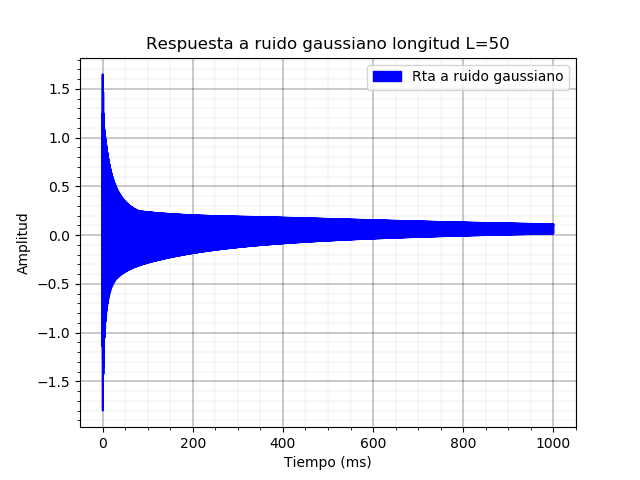
\includegraphics[scale=0.55]{graficos/gaussBloqueS1.png}
	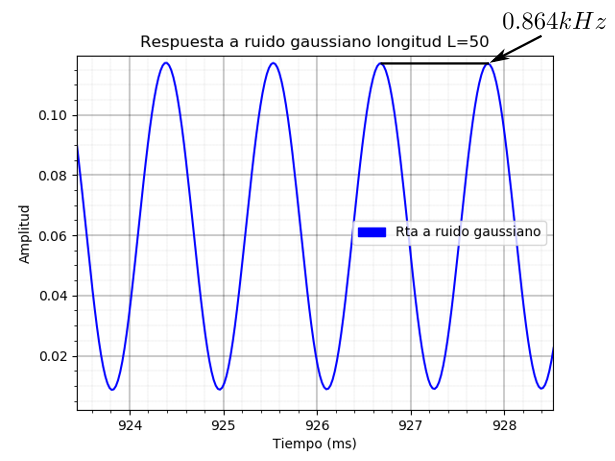
\includegraphics[scale=0.41]{graficos/gaussBloqueS1zoom.png}
	\caption{Respuesta a entrada Gaussiana con y sin zoom, $R_L=1$, $L=50$, $f_s=44.1kHz$}
\end{figure}

Se puede ver que la salida fue a la misma frecuencia que en el caso anterior, al mismo tiempo que nuevamente, estuvo montada sobre una continua. No obstante la salida tuvo la posiblidad de tomar valores negativos.

\begin{figure}[H]
	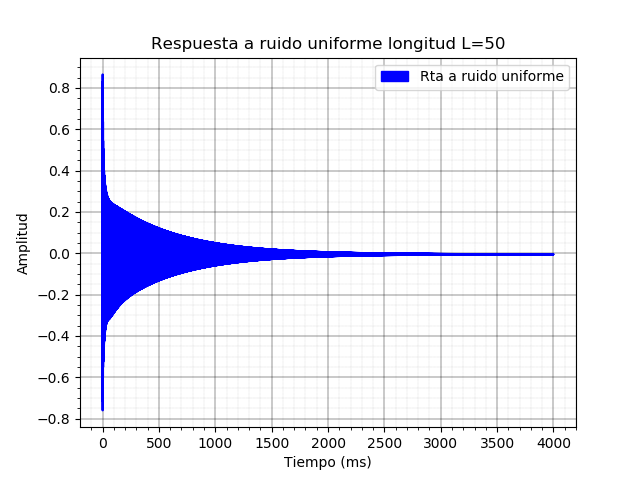
\includegraphics[scale=0.55]{graficos/randomBloqueS1.png}
	\includegraphics[scale=0.55]{graficos/randomBloqueS1zoom.png}
	\caption{Respuesta a entrada de ruido uniforme con y sin zoom, $R_L=1$, $L=50$, $f_s=44.1kHz$}
\end{figure}

Podemos observar que la salida fue similar a la de ruido gaussiano

\subsection{Karplus Strong 2}

\subsubsection{Analisis teórico elemental}
Se estudiará un nuevo sistema con una pequeña modificación la cual consiste en agregar un multiplicador en el bloque realimentador, cuyo valor es aleatorio, puede ser 1 o -1. La probabilidad de que sea 1 se llamará $b$ 
\begin{figure}[H]
	\begin{center}
	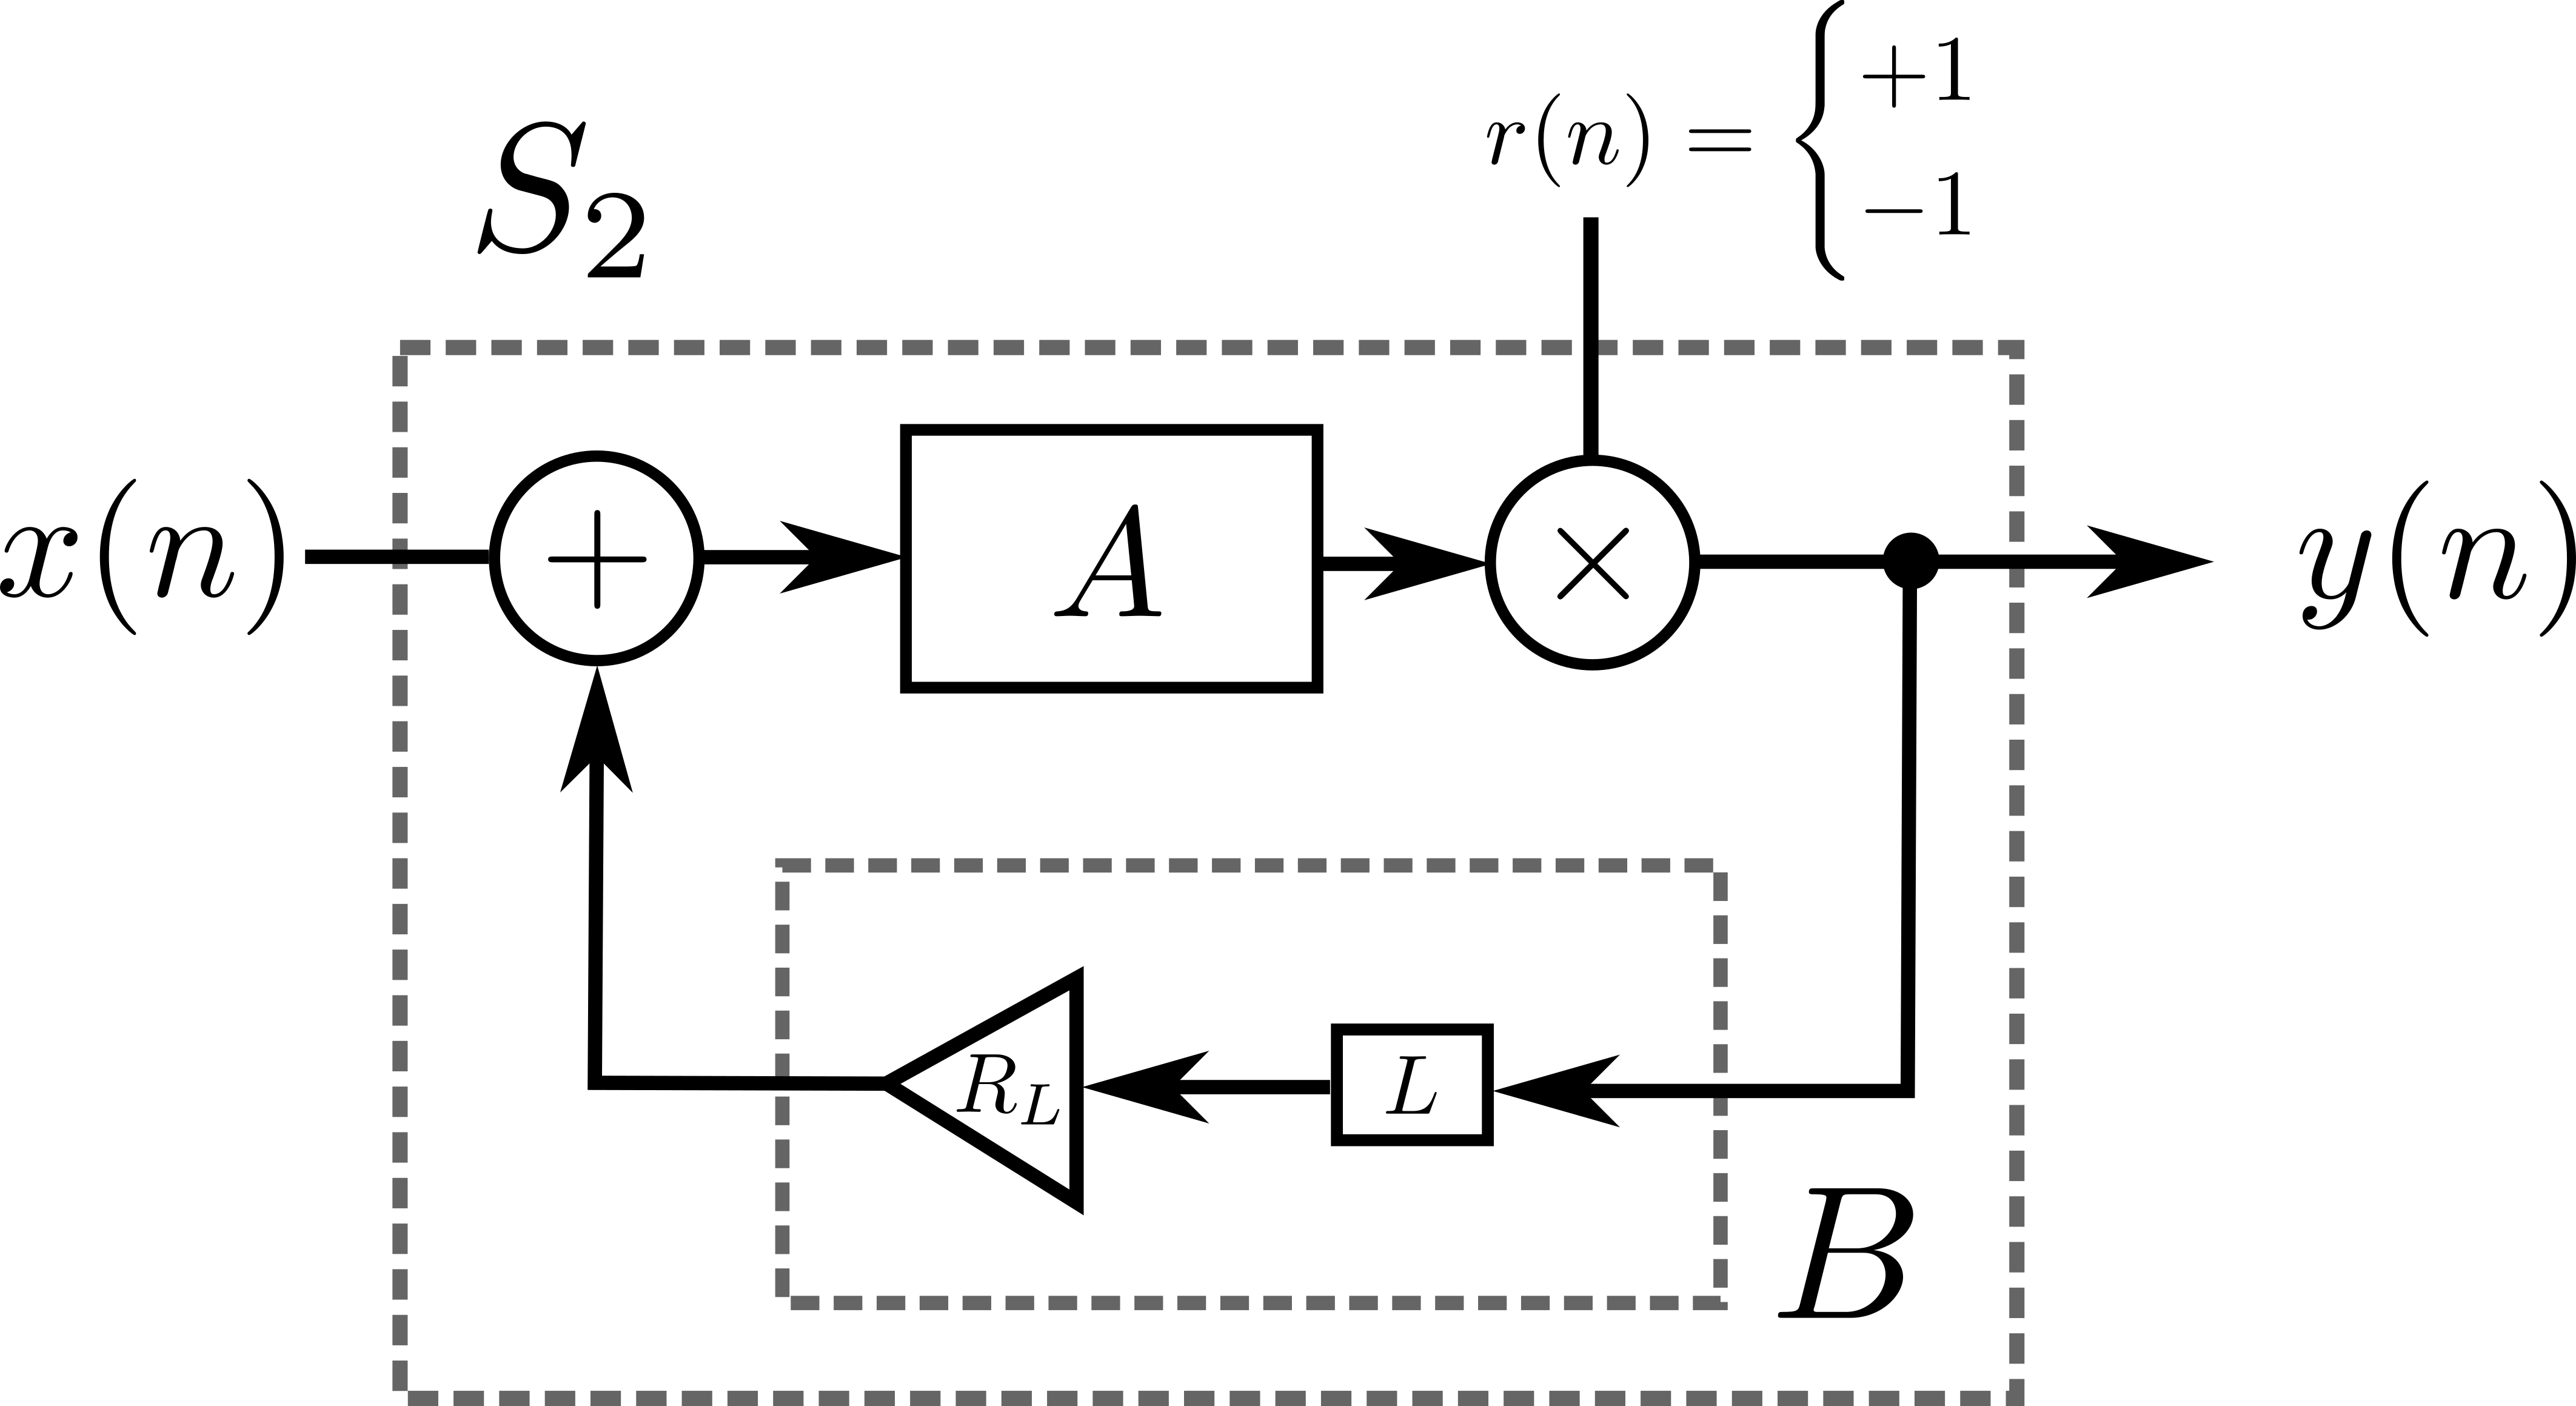
\includegraphics[scale=1]{graficos/bloque3ej5.png}
	\caption{Diagrama del sistema $S_2$}

	\end{center}
\end{figure}

Escrito en lenguaje matemático

\begin{equation}
	A(z)=b(\frac{1}{2}+\frac{1}{2}z^{-1})
\end{equation}
\begin{equation}
	B(z)=\frac{1}{2}z^{-L}
\end{equation}

Usando teória de feedback concluimos que

\begin{equation}
	S_2(z)=\frac{\frac{1}{2}r+\frac{1}{2}rz^{-1}}{1-\frac{1}{2}rR_Lz^{-L}-r\frac{1}{2}R_Lz^{-L-1}}
\end{equation}
\begin{equation}
	y(n) = \frac{1}{2}rx(n) + \frac{1}{2}rx(n-1) + \frac{1}{2}rR_Ly(n-L)+\frac{1}{2}rR_Ly(n-L-1)
\end{equation}
Observamos de la ecuación de diferencias que el sistema es prácticamente equivalente al anterior con una diferencia; ahora la salida se invierte de manera aleatoria ciclo a ciclo. Esta aleatoriedad ayudará a simular la aleatoriedad de un sonido percutido.
\subsubsection{Respuesta en frecuencia}

Debido a la complejidad trigonometricá del cálculo exacto se opto por aproximar númericamente el gráfico de $\phi(w)=\angle H(e^{jw})$ (respuesta en frecuencia del sistema) 
Por otro lado se decidió tampoco realizar el cálculo de la frecuencia de resonancia con exactitud, debido a su elevada complejidad. En realidad no es estrictamente necesario, en realidad en la práctica cuando $b$ sea distinto de 1 o 0 ocurrira notable interferencia en el lazo que destruira la resonancia; lo cual provocará que el sonido se extinga luego de breves instantes.

Ahora se mostrará la respuesta en frecuencia con $b=1, b=\frac{1}{2}, b=0$. Es importante observar que dado que la salida es estrictamente una variable aleatoria, la respuesta en frecuencia entonces estrictamente también es una variable aleatoria. Se decidió mostrar el valor medio de dicha variable aleatoria.

\begin{figure}[H]
	\begin{center}
	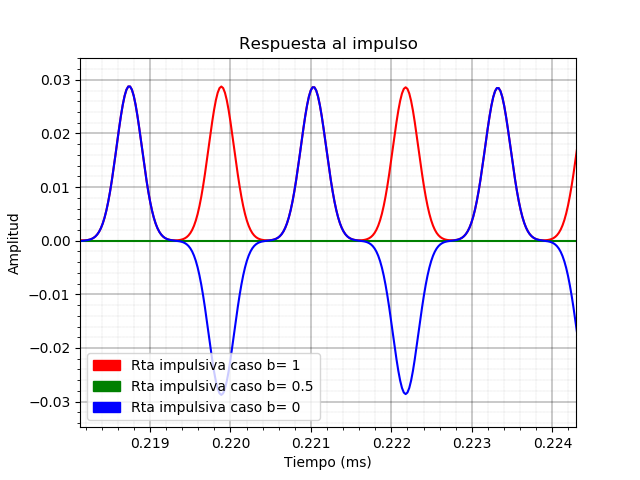
\includegraphics[scale=0.5]{graficos/impulsoB.png}
	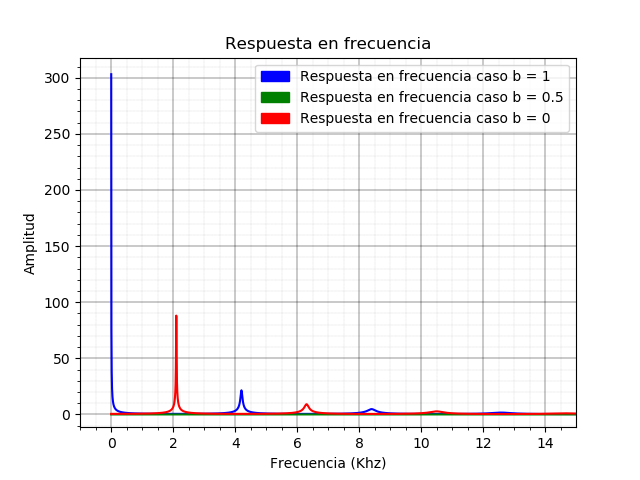
\includegraphics[scale=0.5]{graficos/rtaFreqB.png}
	\caption{Respuesta al impulso y en frecuencia con $b=1, 0.5, 0$ (izquierda a derecha)}

	\end{center}
\end{figure}

Se observa que, como fue predicho, en el caso b=0.5 todas las frecuencias son destruidas luego de un pequeño transitorio. Además, se observó que el caso de b=0 mostró una inversión espectral que provocó que la frecuencia de resonancia se redujerá en dicho casó lo cual implicó un sonido más grave, como el de un arpa.
También se observó una gran amplificación en el caso $b=1$ en la continua. Esto no es un gran problema ya que si la entrada tiene valor medio cercano a 0 y se filtra dicha componente a la salida es un problema evitable.


\section{Sintetización de instrumentos}

En base a las distintas pruebas realizadas anteriormente se procederá a realizar las funciones que permitan sintetizar el sonido de varios instrumentos que son:
\begin{itemize}
	\item Arpa
	\item Guitarra
	\item Tambor (percusión)
\end{itemize}

\subsection{¿Como tener libertad con la frecuencia fundamental?}

La primera necesidad fue tener la libertad de poder sintetizar un sonido con cualquier frecuencia que se necesite. La solución fue sencilla; consistió en modificar el bloque $A$ para que nos permita una mayor libertad al elegir la frecuencia
\begin{figure}[H]
	\begin{center}
	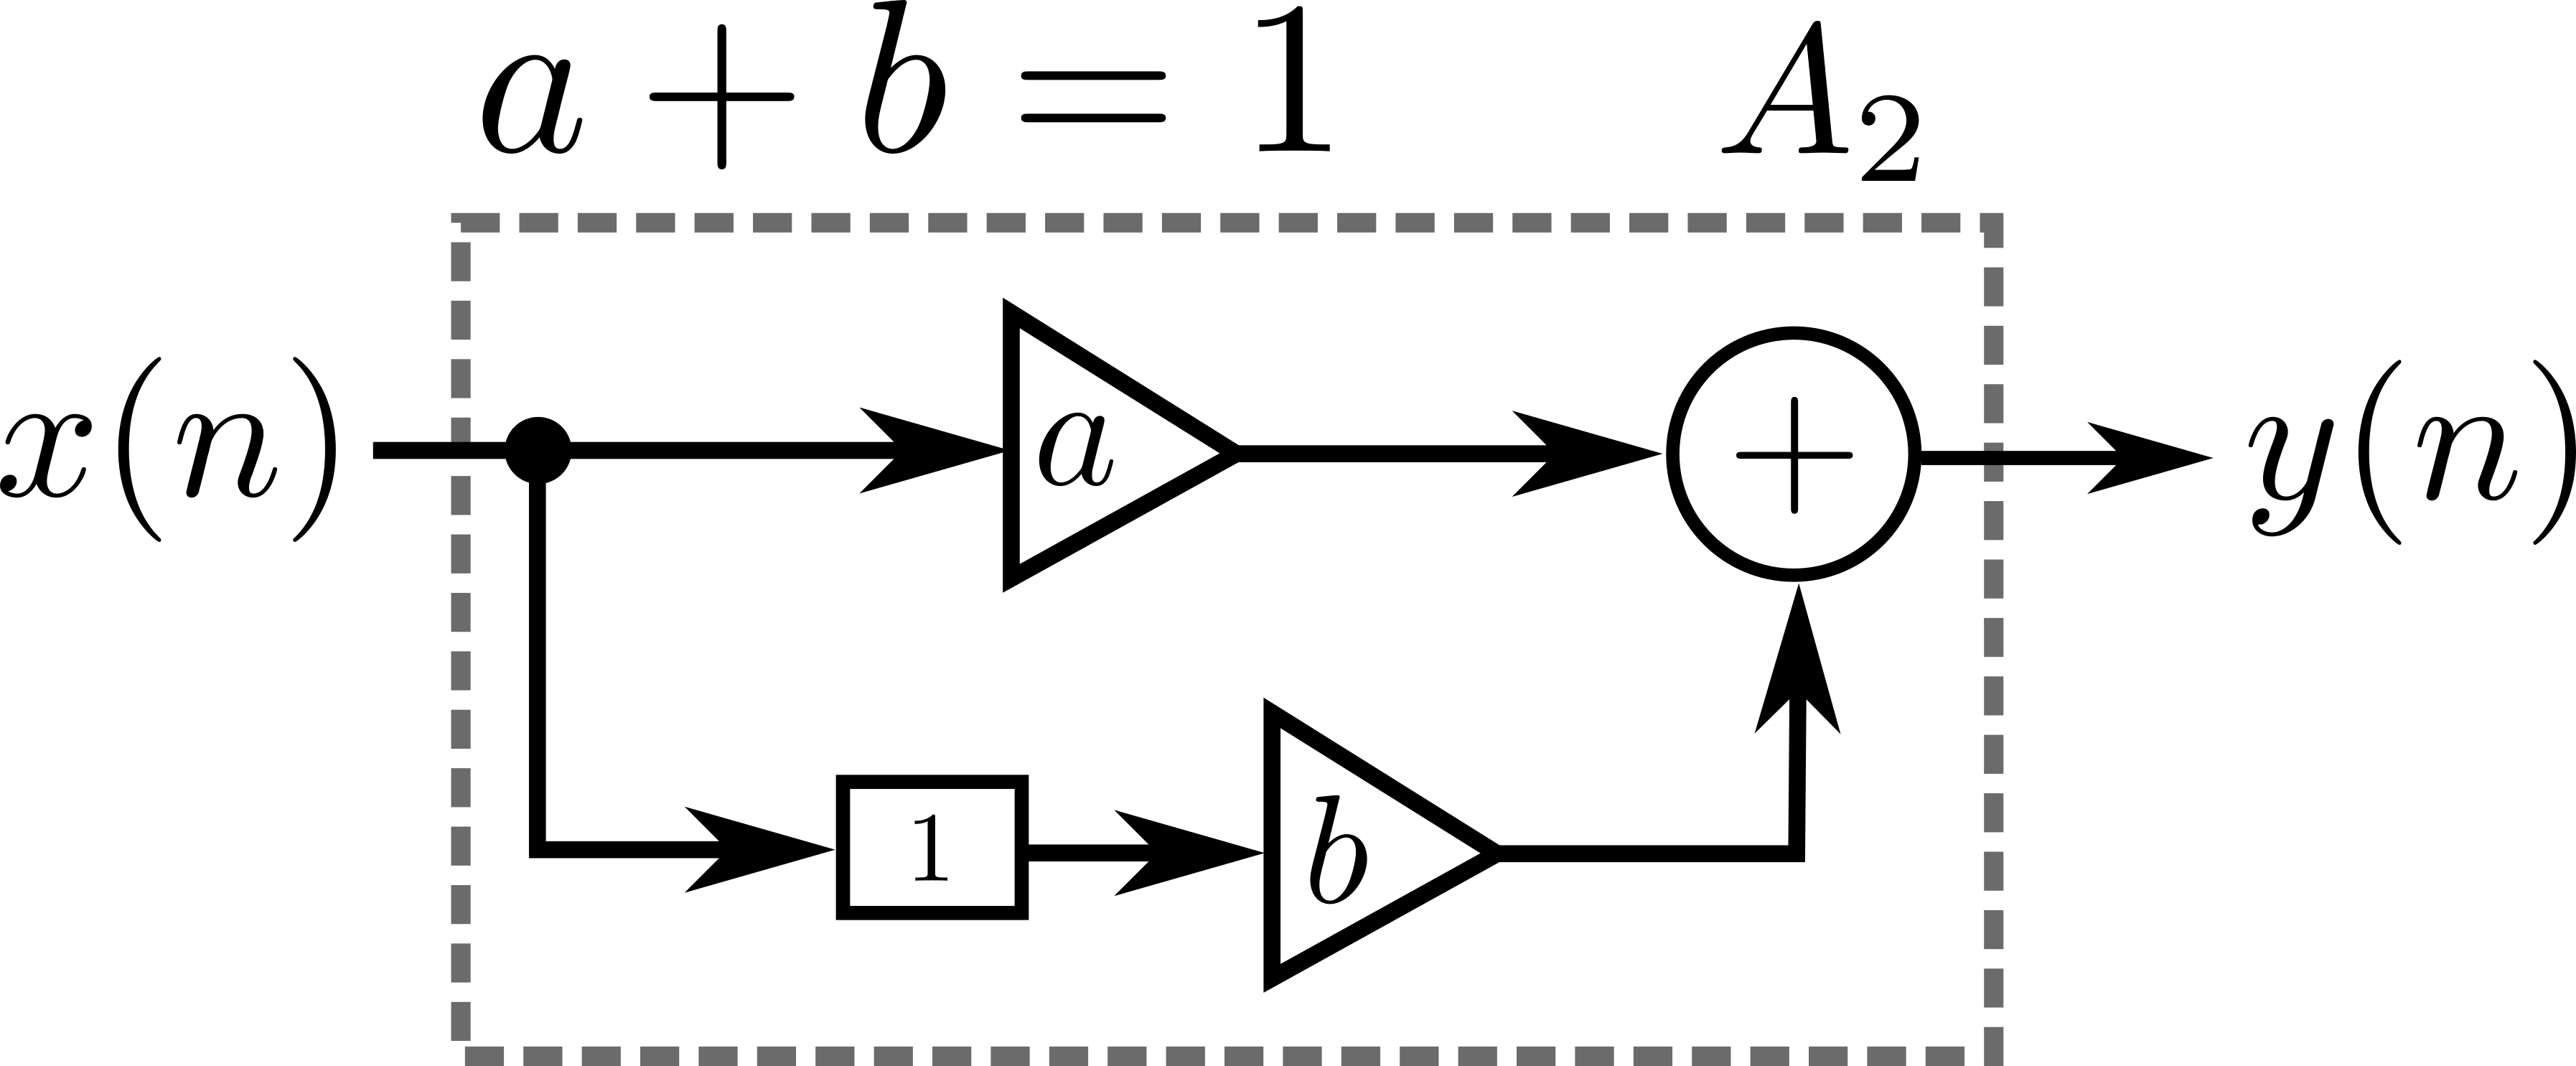
\includegraphics[scale=1]{graficos/bloque4ej5.png}
	\caption{Modificación bloque $A$ para poder personalizar la frecuencia}

	\end{center}
\end{figure}

Con la nueva modificación la frecuencia de resonancia paso a estar dada por

\begin{equation}
	F_R=F_s(a\frac{L}{2}+b\frac{L+1}{2})
\end{equation}

Eligiendo $L$ adecuadamente se puede garantizar que existan $a$ y $b$ entre 0 y 1 que verifiquen la ecuación anterior


\subsection{Sintetización de guitarra}
Se implemento el sonido de una guitarra utilizando el modelo Karplus Strong utilizando la modificación que permitió una elección continua de frecuencias. Los resultados fueron satisfactorios


\subsection{Distorsión del sonido de guitarra}
Se distorsionó el sonido de una guitarra utilizando una modificación al modelo. Se colocó un valor de $R_L>1$ pero, utilizando una funcion normalizadora (entre -1 y 1) se conformó un control automatico de ganancia que evitó la inestabilidad del sistema. Colocando diversos valores de $R_L$ se armó distorsión de distintos tipos. 
 
 
\subsection{Sintetización de instrmento de percusión}

Utilizando la modificación del modelo de Karplus Strong la cuál establecia una variable aleatoria se Sintetizó sonido de instrumentos de percusión. Los resultados fueron satisfactorios


\end{document}